\documentclass{beamer}
\usetheme{Madrid}
\usecolortheme{spruce}

\usepackage{pgfplots}

\usepackage{bm}

\usepackage{color}

\usepackage{graphicx}

\graphicspath{{./img/}}

\title{Stochastic Gradient Descent}
\subtitle{STAT 672 Project}
\author{Tom Wallace}
\institute{George Mason University}
\date{Spring 2018}


\begin{document}

\frame{\titlepage}

%%%%%%%%%%%%% Introduction %%%%%%%%%%%%%%

\begin{frame}
	\frametitle{Estimating model coefficients requires optimization}
	We typically fit statistical models to maximize some measure of goodness
	(e.g., likelihood) or minimize some measure of badness (e.g., risk)
	\\~\\

	Parametric assumptions can make this optimization ``nice'' \\~\\

	OLS has a closed form solution: $\hat{\bm{\beta}} =
	(\bm{X}'\bm{X})\bm{X}'\bm{Y}$ \\~\\

	GLM often uses Newton's method
	\begin{itemize}
		\item \small Knowing the PDF makes finding the
			Hessian (2nd order derivatives) not too onerous \\~\\
	\end{itemize}

\end{frame}

\begin{frame}
	\frametitle{Non-parametric \& high-dimensional settings}
	Suppose that we have a typical supervised classification problem
	\begin{itemize}
		\item \small Non-parametric: no assumptions about distribution of data
		\item Feature vector $\mathbf{X}_i$, label $Y_i$
		\item Want to find best prediction function $f^*(\bm{w}; \bm{X})$ from
			hypothesis class $\mathcal{F}$
		\item Optimization: pick weights $\hat{\bm{w}}$ that minimize
			empirical risk according to some convex
			loss function \\~\\
	\end{itemize}

	Some familiar tools for finding $\hat{\mathbf{w}}$ no longer work well
	\\~\\

	But we still know that if $L$ is convex, there is a unique global
	minimum, and the gradient at that point must be 0 \\~\\

	Gradient descent is a numerical strategy to search for that point
\end{frame}

\begin{frame}
	\frametitle{Gradient descent is an iterative search procedure}
	\begin{figure}[h]
	\centering
	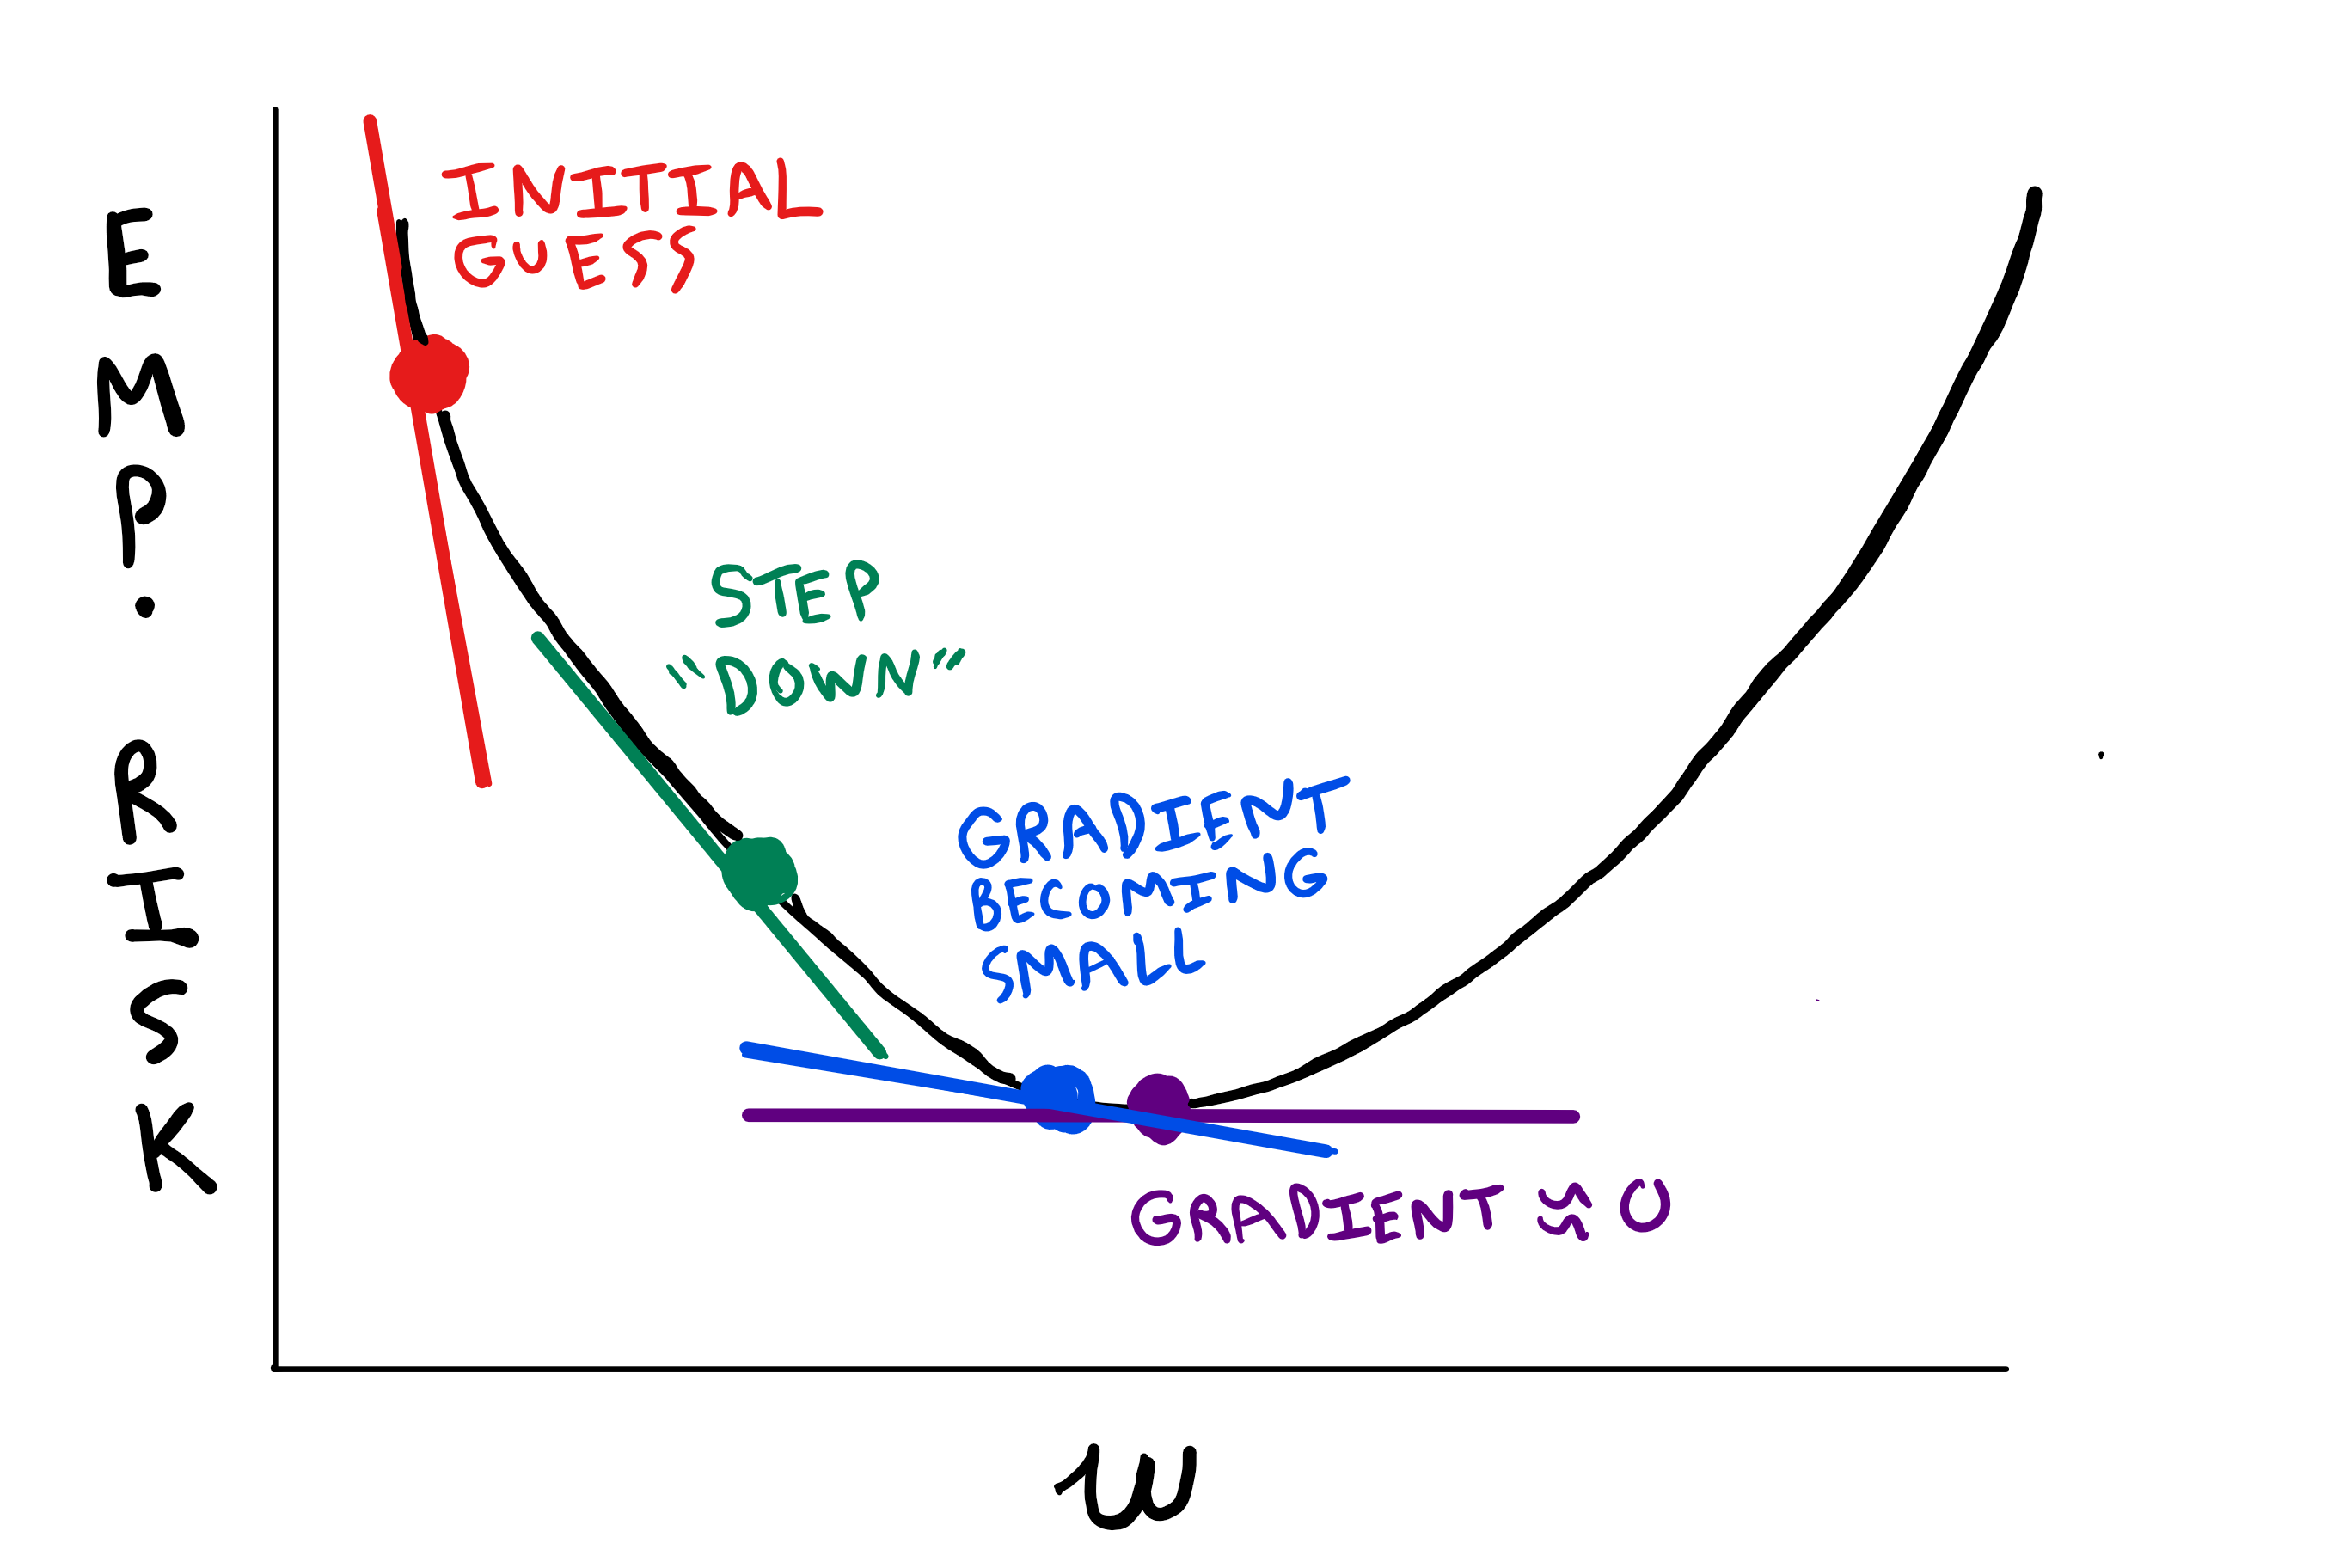
\includegraphics[scale=0.33]{Sketch}
	\end{figure}
\end{frame}

\begin{frame}
	\frametitle{A more formal explanation}

	$\mathbf{w}^{(t+1)} = \mathbf{w}^{(t)} - \gamma \frac{1}{n}\sum_{i=1}^n
	\nabla_w L(f(\bm{w}^{(t)}; \mathbf{X}_i), Y_i)$ \\~\\

	Stop if gradient $\leq \epsilon$ \\~\\

	Step size $\gamma$ can vary over time \\~\\

\end{frame}

\begin{frame}
	\frametitle{Batch gradient descent is computationally expensive}
	In ``plain'' (batch) gradient descent, for \textcolor{red}{every step}, 
	we have to evaluate the gradient at \textcolor{blue} {every observation}

	$$
	\textcolor{red}{\mathbf{w}^{(t+1)}} = \mathbf{w}^{(t)} - \gamma \frac{1}{n}
	\textcolor{blue}{\sum_{i=1}^n}
	\nabla_w L(f(\bm{w}^{(t)}; \mathbf{X}_i), Y_i)
	$$\\~\\

	This becomes computationally intractable as $n$ grows large 
	\begin{itemize}
		\item \small If $n$ = 10 million, have to evaluate 
			gradient 10 million times every step
	\end{itemize}
\end{frame}

\begin{frame}
	\frametitle{Stochastic gradient descent (SGD) takes less time}

	For each step, gradient is computed for a \textcolor{red}{single} randomly
	chosen observation $i$:

	$$
	{\mathbf{w}^{(t+1)}} = \mathbf{w}^{(t)} - \gamma \nabla_w
	L(f(\bm{w}^{(w)}; \mathbf{X}_{\textcolor{red}{i}}), Y_{\textcolor{red}{i})}
	$$ \\~\\

	This simplification makes approximation much ``noisier'', and hence SGD
	requires more iterations \\~\\

	But, each iteration is faster and so SGD can reach a predefined
	level of risk or error in less time
\end{frame}

\begin{frame}
\frametitle{SGD is noisier than batch GD}
	\centering
	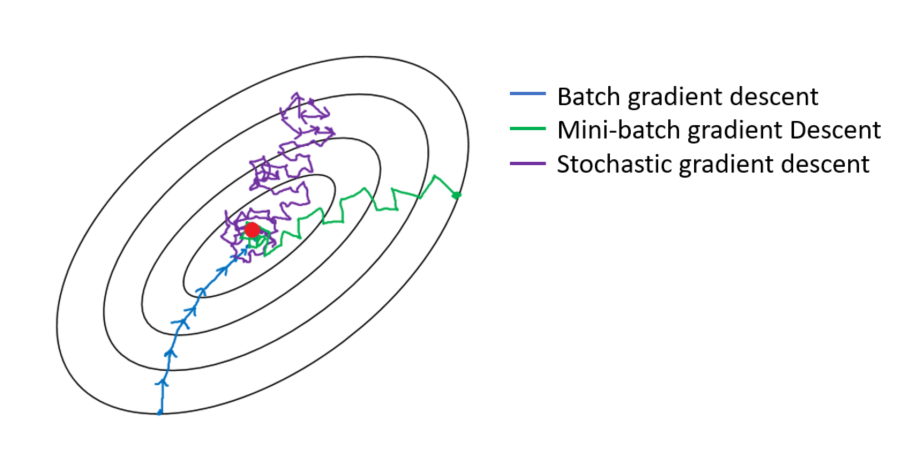
\includegraphics[scale=0.3]{noise}

	\tiny Source: towardsdatascience.com
\end{frame}

\begin{frame}
	\frametitle{SGD is useful when $n$ is large \& compute
	time is important}
	\begin{table}[t]
		\begin{tabular}{|l|c|c|}
			\hline
			& \textbf{GD} & \textbf{SGD} \\
			\textbf{Time to accuracy} $\mathbf{\rho}$ & $n \log
			\frac{1}{\rho}$ & $\frac{1}{\rho}$ \\
			\hline
		\end{tabular}
	\end{table}

	\begin{figure}
		\caption{Fitting OLS coefficients, $n=10$ million}
	\centering
	\includegraphics[scale=0.35]{speed}
	\end{figure}

			
\end{frame}

\begin{frame}
	\frametitle{SGD is very popular in academia and industry}
	Many, many, \textit{many} statistical learning models use SGD to fit weights \\~\\

	If a Silicon Valley press release uses any of the following phrases...
	\begin{itemize}
		\item \small ``Neural networks''
		\item ``Machine learning''
		\item ``AI'' 
	\end{itemize}

	...SGD probably is involved. \\~\\
	
\end{frame}

\begin{frame}
	\frametitle{Example: Google's \textbf{AlphaGo} program}
	\begin{figure}[b]
	\centering
	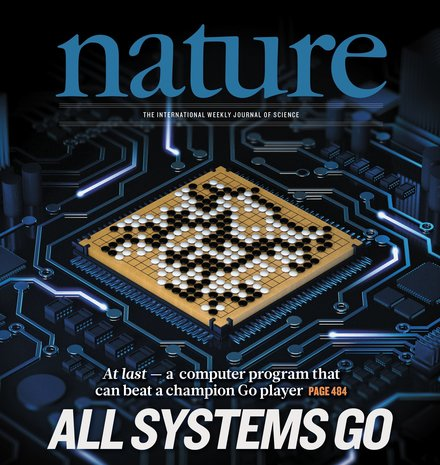
\includegraphics[scale=0.4]{go}
	\end{figure}
\end{frame}

\begin{frame}
	\frametitle{Google slides from ICML 2016}
	\centering
	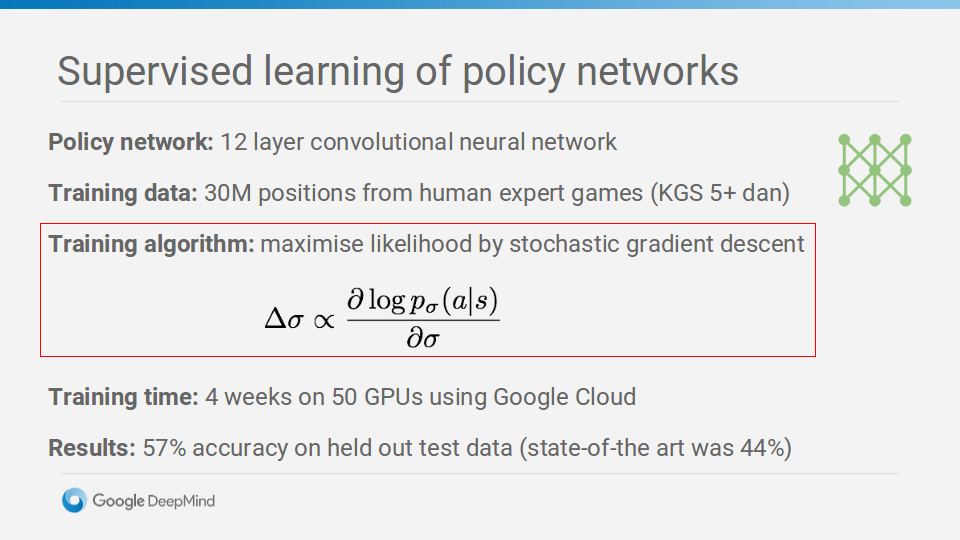
\includegraphics[scale=0.3]{screenshot}
\end{frame}

\end{document}


